\let\negmedspace\undefined
\let\negthickspace\undefined
\documentclass[journal]{IEEEtran}
\usepackage[a5paper, margin=10mm, onecolumn]{geometry}
\usepackage{lmodern} % Ensure lmodern is loaded for pdflatex
\usepackage{tfrupee} % Include tfrupee package

\setlength{\headheight}{1cm} % Set the height of the header box
\setlength{\headsep}{0mm}     % Set the distance between the header box and the top of the text

\usepackage{gvv-book}
\usepackage{gvv}
\usepackage{cite}
\usepackage{amsmath,amssymb,amsfonts,amsthm}
\usepackage{algorithmic}
\usepackage{graphicx}
\usepackage{textcomp}
\usepackage{xcolor}
\usepackage{txfonts}
\usepackage{listings}
\usepackage{enumitem}
\usepackage{mathtools}
\usepackage{gensymb}
\usepackage{comment}
\usepackage[breaklinks=true]{hyperref}
\usepackage{tkz-euclide} 
\usepackage{listings}
\usepackage{gvv}                                        
\def\inputGnumericTable{}                                 
\usepackage[latin1]{inputenc}                                
\usepackage{color}                                            
\usepackage{array}                                            
\usepackage{longtable}                                       
\usepackage{calc}                                             
\usepackage{multirow}                                         
\usepackage{hhline}                                           
\usepackage{ifthen}                                           
\usepackage{lscape}
\begin{document}

\bibliographystyle{IEEEtran}
\vspace{3cm}

\title{6.5.21}
\author{EE24BTECH11005 - Arjun Pavanje}
% \maketitle
% \newpage
% \bigskip
{\let\newpage\relax\maketitle}
\textbf{Question:}
Of all the closed right circular cylindrical cans of given volume  $100 cm^3$, find the dimensions of the can which has minimum surface area \newline
\solution \newline
Surface Area of cylinder is given by, 
\begin{align}
  2\pi rh + 2\pi r^2
\end{align}
where $r$ is the radius of the cylinder, $h$ is the height of the cylinder.\newline
Volume of a cylinder is given by, 
\begin{align}
  \pi r^2 h
\end{align}
where $r$ is the radius of the cylinder, $h$ is the height of the cylinder.\newline
Given that volume is $100 cm^3$,
\begin{align}
  \pi r^2 h = 100\\
  h = \frac{100}{\pi r^2}
\end{align}
Equation $\brak{1}$ becomes,
\begin{align}
  \brak{\frac{200}{r} + 2\pi r^2}
\end{align}
\textbf{Theoretical Solution}\newline
To minimize surface area, differentiate equation $\brak{1}$ and set it to zero,
\begin{align}
  \frac{4\pi r^3 - 200}{r^2}=0
\end{align}
value of $r$ at which satisfies is, $\brak{\frac{50}{\pi}}^{\frac{1}{3}}$. We can verify that this is a minima by differentiating equation $\brak{6}$,
\begin{align}
  \frac{400}{r^3} + 4\pi
\end{align}
Thus we see that at the above value of $r$, it is a minima.\newline
Can of given volume will have maximum surface area when radius is $\brak{\frac{50}{\pi}}^{\frac{1}{3}} cm$, height is $2\brak{\frac{\pi}{50}}^{\frac{1}{3}}$\newline
\textbf{Computational Solution:}\newline
We need to minimize,
\begin{align}
  \brak{\frac{200}{r} + 2\pi r^2}
\end{align}
Applying gradient descent theorem,
\begin{align}
  r_{n+1} = r_n -\mu f^{\prime}\brak{r_n}\\
\end{align}
where $\mu$ is the step size,
\begin{align}
  f^{\prime}\brak{r_n} = -\frac{200}{r_n^2} +4\pi r_n
\end{align}
Final Difference Equation comes out to be, 
\begin{align}
  r_{n+1} = r_n\brak{1 - 4\pi} + \frac{200}{r_n^2} 
\end{align}
Taking inital guess as $2$, step size $0.01$, tolerence as $0.0001$.\newline
We get minimum value of $r$ to be $2.515397787094116 cm \approx \brak{\frac{50}{\pi}}^{\frac{1}{3}} cm$

\textbf{Alternate Computational Solution: }\newline

We can also solve it using $cvxpy$ module in python. On running the code we get,\newline
Minimum value of $r$ is, $2.515299390016942 cm$, Minimum surface area is, $ 119.26542080485049 cm^2$

\begin{figure}[h!]
   \centering
   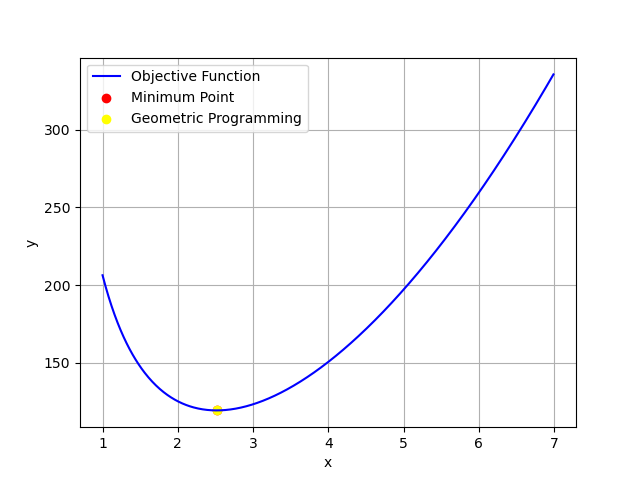
\includegraphics[width=1\columnwidth]{figs/fig.png}
   \caption{Minimizing $\brak{\frac{200}{r} + 2\pi r^2}$. Surface Area function with point of minima}
   \label{stemplot}
\end{figure}
\end{document}
